
\def \Subject {محاسبه دستی یک مرحله آموزش شبکه عصبی}
\def \Session { یک}
% \setcounter{chapter}{\Session-1}
\renewcommand{\chaptername}{سوال}
\chapter{\Subject}
این سوال به محاسبات مورد نیاز در یک شبکه عصبی و همچنین تاثیر بخش‌های مختلف یک شبکه بر خروجی می‌پردازد.
\section{محاسبه دستی یک شبکه عصبی}
در این بخش باید قسمت رو به جلو و رو به عقب یک شبکه MLP حساب شود. معماری شبکه در شکل 
\ref{q1_mlp_architecture}
رسم شده است.
\begin{figure}[H]
\centering

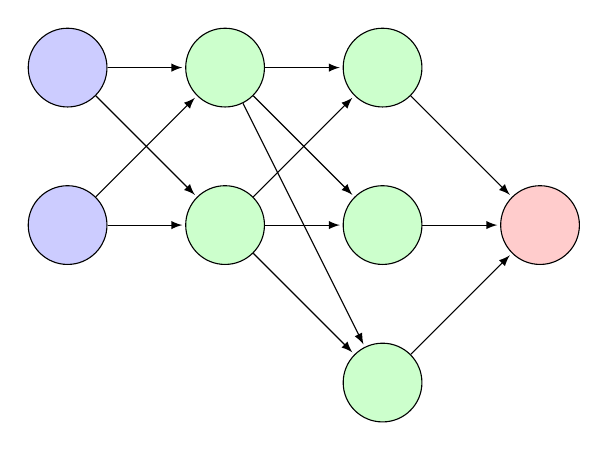
\begin{tikzpicture}[shorten >=1pt,>=latex,node distance=2cm, auto]
	
	% Define node styles
	\tikzstyle{input node} = [circle, draw, minimum size=1cm, fill=blue!20]
	\tikzstyle{hidden node} = [circle, draw, minimum size=1cm, fill=green!20]
	\tikzstyle{output node} = [circle, draw, minimum size=1cm, fill=red!20]
	
	% Place nodes for layers
	\node[input node] (input1) {};
	\node[input node] (input2) [below of=input1] {};
	
	\node[hidden node] (hidden1) [right of=input1] {};
	\node[hidden node] (hidden2) [below of=hidden1] {};
	
	\node[hidden node] (hidden3) [right of=hidden1] {};
	\node[hidden node] (hidden4) [below of=hidden3] {};
	\node[hidden node] (hidden5) [below of=hidden4] {};
	
	
	\node[output node] (output1) [right of=hidden4] {};

	  
	  
	% Draw edges between layers
	\foreach \source/\dest in {
		input1/hidden1, 
		input2/hidden1, 
		input1/hidden2, 
		input2/hidden2, 
		hidden1/hidden3,
		hidden1/hidden4,
		hidden1/hidden5,
		hidden2/hidden3,
		hidden2/hidden4,
		hidden2/hidden5,
		hidden3/output1, 
		hidden4/output1, 
		hidden5/output1}
	\path (\source) edge[->] (\dest);
	
\end{tikzpicture}
\caption{معماری شبکه ذکر شده در سوال. گره‌های آبی ورودی، گره‌های سبز لایه‌های پنهان و گره قرمز لایه خروجی است.}
\label{q1_mlp_architecture}
\end{figure}


اطلاعات شبکه نیز بصورت زیر است (برای مقدار $b_2$ چون فقط یک عدد صفر در سوال آمده است، فرض شده است آن مقدار برای همه نورون ها است):
\begin{latin}
	~\\
	$
	x = \begin{bmatrix}
			1 \\
			0.5 
		\end{bmatrix}
	w_1 = \begin{bmatrix}
		1 & 0  \\
		-1 & 1 
	\end{bmatrix}
	b_1 = \begin{bmatrix}
		0 \\
		0.5
	\end{bmatrix}
	w_2 = \begin{bmatrix}
		0 & -2 & -1 \\
		1 & 1 & 1
	\end{bmatrix}
	b_2 = \begin{bmatrix}
		0 \\
		0 \\
		0
	\end{bmatrix}
	w_3 = \begin{bmatrix}
		1 \\
		-1 \\
		1
	\end{bmatrix}
	b_3 = \begin{bmatrix}
		2
	\end{bmatrix}
	learning\_rate = 0.5
	$
\end{latin}
\subsection{انتشار رو به جلو }  
داریم :
\begin{latin}
	~\\
	$
	z_1 = w_1^T x + b_1 = 
	\begin{bmatrix}
		1 & -1  \\
		0 & 1 
	\end{bmatrix}
	\begin{bmatrix}
		1 \\
		0.5 
	\end{bmatrix}
	+ 
	\begin{bmatrix}
		0 \\
		0.5
	\end{bmatrix}
	=
	\begin{bmatrix}
		0.5 \\
		1
	\end{bmatrix}
	\quad 
	a_1 = \sigma(z_1) \approx \begin{bmatrix}
		0.62 \\
		0.73
	\end{bmatrix}
	\\\\
	z_2 = w_2^T a_1 + b_2 = \begin{bmatrix}
		0 & 1 \\
		-2 & 1 \\
		-1 & 1
	\end{bmatrix}
	\begin{bmatrix}
		0.62 \\
		0.73
	\end{bmatrix}
	= \begin{bmatrix}
		0.73 \\
		-0.51 \\
		0.11
	\end{bmatrix}
	\quad 
	a_2 = \sigma(z_2)  = \begin{bmatrix}
		0.67 \\
		0.38 \\
		0.52
	\end{bmatrix}
	\\\\
	z_3 = w_3^T a_2 + b_3  = \begin{bmatrix}
		1 & -1 & 1
	\end{bmatrix}
	\begin{bmatrix}
		0.67 \\
		0.38 \\
		0.52
	\end{bmatrix} 
	+ 
	 \begin{bmatrix}
		2
	\end{bmatrix}
	=  \begin{bmatrix}
		2.81
	\end{bmatrix}
	a_3 = z_3 = 2.81
	\\
	\Rightarrow \hat{y} = 2.81
	$
\end{latin}
\subsection{انتشار رو به عقب}
اول باید مقدار خطا را محاسبه کرد و سپس گرادیان‌ها را حساب کرد. چون از 
\lr{SGD}
استفاده می‌شود، فقط باید همین نمونه را در نظر گرفت. داریم:
\begin{latin}
	~\\
	$
	E = error_{MSE} = (y - \hat{y})^2 = (3.97 - 2.81)^2 = (1.16)^2 \approx 1.35
	\\
	\cfrac{\partial E}{\partial \hat{y}} = 2 (\hat{y}  - y)  = -2.32 
	\\
	\cfrac{\partial \hat{y}}{\partial a_3} = \cfrac{\partial a_3}{\partial z_3} = 1
	\\
	\delta_i = \cfrac{\partial E}{\partial z_i} = 
	\cfrac{\partial E}{\partial z_{i + 1}} * \cfrac{\partial z_{i + 1}}{\partial a_i} * \cfrac{\partial a_{i}}{\partial z_i} 
	= 
	 W_{i + 1} \delta_{i + 1}  \odot \sigma^{'} (z_i) 
	\\
	\cfrac{\partial E}{\partial b_i} = \delta_i 
	\quad 
	\cfrac{\partial E}{\partial W_i} = (  a_{i - 1} \delta_i^T ) \text{ or }( x \delta_i^T)
	$
\end{latin}
{

%	\\
%	\cfrac{\partial z_3}{b_3} = \begin{bmatrix}
%		1
%	\end{bmatrix}
%	\\
%	\cfrac{\partial z_3}{w_3} = a_2
%	\\
%	\cfrac{\partial z_3}{a_2} = w_3^T
%	\\
%	\cfrac{\partial a_2}{z_2} = a_2 (1 - a_2)
%	\\
%	\cfrac{\partial z_2}{\partial b_2} = 1
%	\\
%	\cfrac{\partial z_2}{\partial w_2} = a_1
%	\\
%	\cfrac{\partial z_2}{\partial a_1} = w_2^T
%	\\ 
%	\cfrac{\partial a_1}{\partial z_1} = a_1 (1 - a_1)
%	\\
%	\cfrac{\partial z_1}{b_1} = 1
%	\\
%	\cfrac{z_1}{w_1} = x
%	$
%\end{latin}
%طبق قاعده زنجیری داریم:
%\begin{latin}
%	~\\
%	$
%	\cfrac{\partial E}{\partial b_3} = 
%	\cfrac{\partial E}{\partial \hat{y}} * \cfrac{\partial \hat{y}}{\partial a_3} * \cfrac{\partial a_3}{\partial z_3}   * \cfrac{\partial z_3}{\partial b_3} = -2.32
%	\\
%	 \cfrac{\partial E}{\partial w_3} = 
%	 \cfrac{\partial E}{\partial \hat{y}} * \cfrac{\partial \hat{y}}{\partial a_3} * \cfrac{\partial a_3}{\partial z_3}   * \cfrac{\partial z_3}{\partial w_3} = -2.32 * a_2
%	 \\
%	 \cfrac{\partial E}{\partial b_2} = 
%	 \cfrac{\partial E}{\partial \hat{y}} * \cfrac{\partial \hat{y}}{\partial a_3} * \cfrac{\partial a_3}{\partial z_3}   * \cfrac{\partial z_3}{\partial a_2} * \cfrac{\partial a_2}{\partial z_2} * \cfrac{\partial z_2}{\partial b_2}
%	 =
%	 -2.32 * w_3^T \odot (a_2 ) (1 - a_2) 
%	 \\
%	 \cfrac{\partial E}{\partial w_2} = 
%	 \cfrac{\partial E}{\partial \hat{y}} * \cfrac{\partial \hat{y}}{\partial a_3} * \cfrac{\partial a_3}{\partial z_3}   * \cfrac{\partial z_3}{\partial a_2} * \cfrac{\partial a_2}{\partial z_2} * \cfrac{\partial z_2}{\partial w_2}
%	 =
%	 -2.32 * w_3^T \odot (a_2 ) (1 - a_2)  * a_1
%	 \\
%	 \cfrac{\partial E}{\partial w_2} = 
%	\cfrac{\partial E}{\partial \hat{y}} * \cfrac{\partial \hat{y}}{\partial a_3} * \cfrac{\partial a_3}{\partial z_3}   * \cfrac{\partial z_3}{\partial a_2} * \cfrac{\partial a_2}{\partial z_2} * \cfrac{\partial z_2}{\partial w_2}
%	=
%	-2.32 * w_3^T \odot (a_2 ) (1 - a_2)  * a_1	 
%	\\
%	\cfrac{\partial E}{\partial b_1} = 
%	\cfrac{\partial E}{\partial \hat{y}} * \cfrac{\partial \hat{y}}{\partial a_3} * \cfrac{\partial a_3}{\partial z_3}   * \cfrac{\partial z_3}{\partial a_2} * \cfrac{\partial a_2}{\partial z_2} * \cfrac{\partial z_2}{\partial a_1} * \cfrac{\partial a_1}{\partial z_1} *  \cfrac{\partial z_1}{\partial b_1}
%	= 
%	-2.32 * w_3^T \odot (a_2 ) (1 - a_2)  * w_2^T \odot (a_1) (1 - a_1)
%	\\
%	\cfrac{\partial E}{\partial w_1} = 
%	\cfrac{\partial E}{\partial \hat{y}} * \cfrac{\partial \hat{y}}{\partial a_3} * \cfrac{\partial a_3}{\partial z_3}   * \cfrac{\partial z_3}{\partial a_2} * \cfrac{\partial a_2}{\partial z_2} * \cfrac{\partial z_2}{\partial a_1} * \cfrac{\partial a_1}{\partial z_1} *  \cfrac{\partial z_1}{\partial w_1}
%	= 
%	-2.32 * w_3^T \odot (a_2 ) (1 - a_2)  * w_2^T \odot (a_1) (1 - a_1) * x
%	$
%\end{latin}

پس داریم:
\begin{latin}
	~\\
	$
	\delta_3 = \cfrac{\partial E}{\partial z_3} =  \begin{bmatrix}
		-2.32
	\end{bmatrix} 
	\qquad
	\cfrac{\partial E}{\partial b_3} = -2.32
	 \qquad 
	\cfrac{\partial E}{\partial W_3} \approx  \begin{bmatrix}
		-1.55 \\
		 -0.88 \\
		 -1.21
	\end{bmatrix} 
	\\
	\delta_2 =W_{3} \delta_{3}   \odot \sigma^{'} (z_2) =
	 \begin{bmatrix}
		1 \\
		-1 \\
		1
	\end{bmatrix} 
	\begin{bmatrix}
		-2.32
	\end{bmatrix}
	\odot
	\sigma^{'}(
	\begin{bmatrix}
		0.73\\
		-0.51 \\
		0.11
	\end{bmatrix}
	)
	= 
	\begin{bmatrix}
		-2.32 \\
		2.32 \\
		-2.32
	\end{bmatrix}
	\odot 
	\begin{bmatrix}
		0.22 \\
		0.23 \\
		0.25
	\end{bmatrix}
	= 
	\begin{bmatrix}
		- 0.51 \\
		0.53 \\
		-0.58
	\end{bmatrix}
	\\
	\cfrac{\partial E}{\partial b_2} 
	= 
	\begin{bmatrix}
	- 0.51 \\
	0.53 \\
	-0.58
\end{bmatrix}
	\qquad
	\cfrac{\partial E}{\partial W_2} = 
	\begin{bmatrix}
		0.62 \\
		0.73
	\end{bmatrix}
	\begin{bmatrix}
	- 0.51 &
	0.53 &
	-0.58
\end{bmatrix}
	=  
	\begin{bmatrix}
-0.32 & 0.33 & -0.36 \\ 
-0.37 & 0.39 & -0.42 
	\end{bmatrix}
	\\
	\delta_1 = 
		W_2 \delta_2 \odot \sigma^{'}(z_1)
		=
\begin{bmatrix}
	0 & -2 & -1 \\
	1 & 1 & 1
\end{bmatrix}
\begin{bmatrix}
	- 0.51 \\
	0.53 \\
	-0.58
\end{bmatrix}
\odot 
		\begin{bmatrix}
	0.24 \\
	0.2
\end{bmatrix}
=
\begin{bmatrix}
	-0.48\\
	-0.56
\end{bmatrix}
\odot 
\begin{bmatrix}
	0.24 \\
	0.2
\end{bmatrix}
= 
\begin{bmatrix}
	-0.12 \\
-0.11
\end{bmatrix}
\\
\cfrac{\partial E}{\partial b_1} = 
\begin{bmatrix}
	-0.12 \\
	-0.11
\end{bmatrix}
\qquad 
\cfrac{\partial E}{\partial w_1} = 
\begin{bmatrix}
1 \\
0.5
\end{bmatrix}
\begin{bmatrix}
	-0.12 &
-0.11
\end{bmatrix}
=
\begin{bmatrix}
	-0.12 & -0.11 \\
	-0.06 & -0.06
\end{bmatrix}
	$
\end{latin}
حال که مشتق خطا نسبت به هرکدام از پارامترها را داریم، باید مقادیر گرادیان‌ها را در ضریب یادگیری ضرب کرد و با مقدار پارامترها جمع کرد. پس داریم:
\begin{latin}
$
~\\
b_{3_{new}} =
\begin{bmatrix}
	2
\end{bmatrix}
 - \begin{bmatrix}
	-1.16
\end{bmatrix} = \begin{bmatrix}
	3.16
\end{bmatrix}
\\
w_{3_{new}} = \begin{bmatrix}
	1 \\
	-1 \\
	1
\end{bmatrix} -‌ \begin{bmatrix}
 -0.78 \\
-0.44 \\
-0.6
\end{bmatrix}
=
\begin{bmatrix}
	1.78 \\
	-0.56 \\
	1.6
\end{bmatrix}
\\
b_{2_{new}} = b_2 - \begin{bmatrix}
	-0.26 \\
	 0.27 \\
	  -0.29
\end{bmatrix} = \begin{bmatrix}
	0.26 \\
-0.27 \\
0.29
\end{bmatrix}
\\
w_{2_{new}} = \begin{bmatrix}
		0 & -2 & -1 \\
1 & 1 & 1
\end{bmatrix} - \begin{bmatrix}
-0.16 & 0.17 & -0.18 \\ 
-0.19 & 0.2 & -0.21 
\end{bmatrix}
=
\begin{bmatrix}
	0.16 & -2.17 & -0.82 \\ 
	1.19 & 0.8 & 0.79 
\end{bmatrix}
\\
b_{1_{new}} = 
\begin{bmatrix}
	0 \\
	0.5
\end{bmatrix} -
\begin{bmatrix}
	-0.06 \\
-0.06
\end{bmatrix}
= 
\begin{bmatrix}
	0.06 \\
0.56
\end{bmatrix}
\\
w_{1_{new}} 
=
\begin{bmatrix}
	1 & 0  \\
	-1 & 1 
\end{bmatrix}
-
\begin{bmatrix}
	-0.06 & -0.06 \\
	-0.03 & -0.03 
\end{bmatrix}
=
\begin{bmatrix}
	1.06 & 0.06 \\
	-0.97 & 1.03
\end{bmatrix}
$
\end{latin}

\section{دلیل استفاده از تابع فعال‌ساز}
اگر از تابع فعال‌ساز استفاده نشود و یا تابع فعال‌ساز یک تابع خطی باشد، عملا استفاده از لایه‌های بیشتر و شبکه عمیق‌تر فرقی با یک شبکه تک لایه نخواهد داشت. 

\begin{equation}
	z_2 = W_2 a_1 + b_2 = W_2 (W_1 x + b_1) + b_2 = W_2 W_1 x + W_2 b_1 + b_2
		\label{shallow_deep_q1}
\end{equation}
{
\small
در فرمول 
\eqref{shallow_deep_q1}
می‌توان دید اگر تابع فعال‌ساز نباشد، این شبکه دولایه عملا معادل با یک شبکه تک لایه است که در آن 
$w_1$
برابر با 
$w_2 w_1$
در شبکه اصلی است و 
$b_1$
برابر با 
$w_2 b_1 + b_2$
در شبکه اصلی است.
}

\section{مشکلات سیگموئید }

\begin{enumerate}
	\item 
	چون مشتق سیگوئید 
	\LTRfootnote{Sigmoid}
	در نواحی دور از صفر به صفر میل می‌کند و مقدار آن بسیار کم است، عملا به روزرسانی وزن‌ها با سرعت کمی انجام می‌شود و زمان آموزش مدل زیاد می‌شود.
	\item 
	چون خروجی بین صفر و یک است و مشتق نیز همواره مثبت است، در به روزرسانی وزن‌ها، گرادیان‌ها هم‌علامت می‌شوند. این موضوع باعث می‌شود که دقت مدل به شدت به وزن‌دهی اولیه وابسته شود و اگر وزن‌دهی اولیه خوب نباشد چون گرادیان‌ها نیز هم‌علامت هستند، به روزرسانی باعث دور شدن از جواب شود (حداقل در آن لایه)
\end{enumerate}

\section{نحوه محاسبه گرادیان رلو}
تابع رلو
\LTRfootnote{ReLU}
یک تابع دوضابطه‌ای است. پس برای مشتق گرفتن از آن باید مشتق هر ضابطه را گرفت و مشتق تابع رلو در بازه ضابطه برابر با مشتق آن ضابطه خواهد بود.

\begin{equation}
	\sigma(x) = 
		\begin{cases}
		0& (x \leq 0) \\
		x &(x > 0)
	\end{cases}
	\label{eq:relu_formula}
\end{equation}

تعریف تابع رلو در 
\eqref{eq:relu_formula}
آمده است. با مشتق گرفتن از هر ضابطه و درنظر گرفتن شرط آن می‌توان گفت:

\begin{equation}
	\sigma^{'}(x)
	=
	\begin{cases}
	0& (x \leq 0) \\
	1 &(x > 0)
		\end{cases}
		=
		U(x)
\end{equation}
که این همان تعریف تابع پله است.